%\documentclass[twocolumn]{article}
%\usepackage[utf8]{inputenc}
%\documentclass[10pt,journal,onecolumn]{IEEEtran}
%\documentclass[10pt,journal,compsoc]{IEEEtran}
\documentclass[10pt, journal, letterpaper]{IEEEtran}
%\documentclass[10pt,journal,compsoc]{IEEEtran}

% NB hyperref package may need to be commented for Latex upload
\usepackage{cite}
%\ifCLASSOPTIONcompsoc
%\ifCLASSINFOpdf
% \usepackage[pdftex]{graphicx}
% declare the path(s) where your graphic files are
% \graphicspath{{../pdf/}{../jpeg/}}
% and their extensions so you won't have to specify these with
% every instance of \includegraphics
% \DeclareGraphicsExtensions{.pdf,.jpeg,.png}
%  \usepackage[nocompress]{cite}
%  \else
% normal IEEE
%  \usepackage{cite}
%  \fi

%  \ifCLASSINFOpdf

%  \else
%\fi
%important package
\usepackage{multirow} 
\usepackage{algpseudocode}
\usepackage{algorithm}
\usepackage{rotating}
\usepackage{kantlipsum} %with the next two command (commath, allowdisplaybreaks) -> allow to break the formulas along the pages
\usepackage{commath}
\allowdisplaybreaks
\usepackage{mathtools}  %with the next command adjust the vertical space between formulas
%\setlength{\jot}{5pt}
%\usepackage{ragged2e}   %if add \justify at each line, that line would be justified. This is used because the abstract of transaction style is not justified  ---- it is not compatible with twocolumn-IEEETrans
%not important
\usepackage{verbatim}
\usepackage{xr-hyper} 
\usepackage{enumitem}
\usepackage{multirow}
\usepackage[table,xcdraw]{xcolor}
\usepackage{array,arydshln}
\usepackage{graphicx,booktabs}
\usepackage{longtable}
%strikethrough not working when nested in a definition
%\usepackage[normalem]{ulem}
%\usepackage{soul}
%\usepackage{fullpage} 
%%%%%%%%%%%%%%%%%%%%%%%%%%%%%%%%%%%%%%%%%%%%%%%%%%%%%%%%%%%%%%%%%%%%%%%%%%%%%
% hyperref package may need to be commented for Latex upload
%\usepackage[pdfusetitle, pdfauthor={Michael Shell, My institution}]{hyperref}
%%%%%%%%%%%%%%%%%%%%%%%%%%%%%%%%%%%%%%%%%%%%%%%%%%%%%%%%%%%%%%%%%%%%%%%%%%%%%
\usepackage{balance}
\usepackage{flushend}
\usepackage{epstopdf}
\usepackage{wrapfig}
\usepackage{latexsym}
\usepackage{amssymb}
\usepackage{amsthm}
\usepackage{amsfonts}
\usepackage{amsmath} %[cmex10]
%\usepackage{flushend} %********************* This package has a bug: Do no include it
\usepackage{graphicx}
\usepackage{latexsym}
\usepackage{booktabs}
\usepackage[style=base]{caption}
\usepackage{subcaption} %******************* This package has conflict with sufig and subfigure
%\usepackage{subfigure}
%\usepackage{subfig}
\usepackage{breqn}
\newtheorem{thm}{Property}
\newtheorem{thm1}{Theorem}
\newtheorem{thm3}{Proposition}
\newtheorem{thm5}{Remark}
\newtheorem{thm7}{Lemma}
\algnewcommand\algorithmicinput{\textbf{INPUT:}}
\algnewcommand\INPUT{\item[\algorithmicinput]}
\algnewcommand\algorithmicoutput{\textbf{OUTPUT:}}
\algnewcommand\OUTPUT{\item[\algorithmicoutput]}
\usepackage[table]{xcolor}
%\usepackage[dvipsnames]{xcolor}
%\usepackage[cmyk]{xcolor}
%\usepackage{natbib}
\usepackage{graphicx}
\usepackage{mathtools}
\usepackage{enumitem,kantlipsum}
\usepackage{adjustbox}
% change the width and height of rows and columns in Tables
\usepackage[thinlines]{easytable}

\algdef{SE}[DOWHILE]{Do}{doWhile}{\algorithmicdo}[1]{\algorithmicwhile\ #1}
\makeatletter
\algnewcommand{\LineComment}[1]{\Statex \hskip\ALG@thistlm \texttt{#1}}
\makeatother
\newcommand{\export}{Exportation\xspace}
\newcommand{\move}{Move\xspace}
\newcommand{\ouralgorithm}{GPE\xspace} %%Green path exportation

\newlength\mylength
\setlength\mylength{\dimexpr.13\columnwidth-1\tabcolsep-0.2\arrayrulewidth\relax}
\usepackage{color}
% we need a better fix for this, see https://tex.stackexchange.com/questions/64298/error-with-xcolor-package
\colorlet{BLUE}{blue}
\usepackage{colortbl}
\definecolor{LightCyan}{RGB}{155, 227, 247}
%\captionsetup[figure]{belowskip=-8pt}
%in test

%\usepackage{nomencl}
%\makenomenclature
%% This code creates the groups
% -----------------------------------------
%\usepackage{etoolbox}
%\renewcommand\nomgroup[1]{%
%	\item[\bfseries
%	\ifstrequal{#1}{P}{Parameters}{%
%		\ifstrequal{#1}{V}{Variables}{%
%			\ifstrequal{#1}{I}{Indices}{%
%				\ifstrequal{#1}{B}{Binary~Variables}{}}}}%
%	]}

% To remove all comments, comment out the definition and use the commented-out
% empty definition below
% otherwise you can comment the line \commentsontrue 
\newcommand{\commentBy}[3]{\textcolor{#1}{\textbf{#2:} #3}}
%\newcommand{\commentBy}[3]{\ignorespaces}

\newif\ifcommentson
%uncomment the line below to show comments
%\commentsontrue

%\newcommand{\ss}[1]{\ifcommentson \commentBy{green}{SS}{#1} \fi}
%\newcommand{\lc}[1]{\ifcommentson \commentBy{blue}{LC}{#1} \fi}
%\newcommand{\mm}[1]{\ifcommentson \commentBy{orange}{MM}{#1} \fi}

\newif\ifextended
\newif\ifshortver

%%% Show only short version in black
%%%        \shorvetrue 
%%%        %\extendedtrue 

%%% Show only extended version in black
%%%        %\shorvetrue 
%%%        \extendedtrue 

%%% Show short version in blue and extended version in purple
%%%        \shorvetrue 
%%%        \extendedtrue 

\shortvertrue
%\extendedtrue

\newcommand{\extended}[1]{\ifextended \ifshortver \textcolor{purple}{#1} \else \textcolor{black}{#1} \fi  \fi}
\newcommand{\shortver}[1]{\ifshortver \ifextended \textcolor{blue}{#1} \else \textcolor{black}{#1} \fi \fi}

%\newcommand{\optional}[1]{#1}
%\newcommand{\optional}[1]{\textcolor{Orange}{#1}}
\newcommand{\optional}[1]{\ignorespaces}


\newif\ifrevisionactive
\newif\ifshowdeleted
\revisionactivetrue
%\showdeletedtrue

\newcommand{\revised}[1]{\ifrevisionactive \textcolor{blue}{#1} \else \textcolor{black}{#1} \fi}

%\newcommand{\deleted}[1]{\ifrevisionactive \ifshowdeleted \textcolor{red}{\sout{#1}} \else \fi \fi}
\newcommand{\deleted}[1]{\ifrevisionactive \ifshowdeleted \textcolor{orange}{#1} \else \fi \fi}


% correct bad hyphenation here
\hyphenation{net-works fa-ci-li-ta-tes fa-ci-li-ta-te mo-ni-to-ring par-ti-cu-lar pe-ri-o-di-cal-ly mi-ni-mi-zing va-ria-tions de-li-ve-red per-ri-o-di-cal-ly}


\begin{document}
\title{Active Monitoring for Virtual Environments: Real-Time Delay Measurement for SDN-based Networks}
\author{}
%\date{October 2018}
\maketitle	
\begin{abstract}
    In modern networks, the amount of delay-sensitive traffic, such as live video streaming, network gaming, and robot-driven flows, has been increased dramatically. Simultaneously, by the emergence of IoT, the importance of these types of traffic is growing rapidly. Therefore, improving the quality of service based on SLA comes to be an important field of study in networking. As the first step to guarantee a metric is to measure it, delay measurement becomes an important focal point in the field. In many cases, measuring the delay matrix is desired, however, current solutions could not handle it without a huge overhead on the network. In this paper, we propose a solution to measure the delay matrix using a real-time low-overhead approach. In this way, we inject some flows into the network and based on the delay of those flows, the link delay matrix is inferred. To this end, flows and corresponding paths should be selected minimizing the network monitoring overhead. The main challenging issue in this part is to select a combination of flows where solving the resulted n-equation m-unknown leads to a unique delay matrix. We first propose a mathematical formulation, in form of Integer Linear Programming (ILP), of the corresponding problem and thereafter develop a heuristic algorithm to overcome the high computational complexity of existing ILP solvers. In the next step, a meta-heuristic algorithm is proposed to solve the above-mentioned equations and infer the delay matrix. The challenging part of this step is the volatility of links delays. The proposed solution is evaluated over several real-world network topologies using Mini-Net network emulator.
\end{abstract}	
\begin{IEEEkeywords} 
    Active Network Monitoring, Real-Time Measurement, Delay Matrix;
\end{IEEEkeywords}

\section{Introduction}
Due to increasing demand for data communication over computer networks, network administrators have to continually improve the way they manage their resources. One of the most promising technologies that offers many advantages for network management and monitoring is software-defined networking. In this regard, separated control and data plane, provide a powerful solution to manage and monitor network traffic. More precisely, since the controller can get customized statistics from SDN switches it is possible for the controller to view the status of the network from a centralized perspective. Although exploitation of state-of-the-art technologies is inevitable, this is not enough to handle the current requests on the traffic transmission. Consequently, recent networks have to continually improve their networking service by over-estimating the traffic demands to provide proper infrastructure for user data. This will end up increasing the network capacity. This huge bandwidth can serve the increasing demand on traffic bandwidth, however, controlling the network delay below a satisfying value is still a challenging issue. 

The above-mentioned issue attracts more attention in modern networks such as 5G network where there are many delay-sensitive applications. In other words, reducing network communication delay plays an important role in improving service quality. This is because there are many delay-sensitive services such as video streaming, VNF re-placement, multiplayer gaming, factory robots, and self-driving cars. For many of these high bit-rate delay-sensitive traffics, it is critical to have good network performance in order to provide QoS and guarantee an adequate QoE for the end-user. Considering this in mind, delay management receives a great interest in modern computer networks. The first step to manage the delay is to measure it. This can be done through out different approaches based on the main purpose of the measurement. One of the most valuable types of delay measurement is the measurement of the delay matrix. Delay matrix is the real-time matrix of delay between every pair of nodes (every links). 

 There are many applications for delay matrix as some of them are: SLA-aware traffic engineering, Network troubleshooting and diagnostic, Multi-objective Resource Allocation, Providing a platform for clients of virtual network providers to validate if the provider meets the SLA, and Learning Network Behaviour. Regarding SLA-aware traffic engineering, delay matrix is an invaluable input to do QoS-aware traffic engineering. Considering the central resource administration of SDN networks, flows can be routed via low delay and packet loss links using these metrics. There are lots of works using network statistics to provide a SLA-based route such as \cite{tajiki2017optimal,kamoun2018ip,lin2018dte}. Another application of delay matrix is in network troubleshooting and diagnostic. Due to distributed nature of networks, troubleshooting is extremely hard. Many failures are considered as network ''problems" while they are not. Researches show that about 50$\%$ of these “network” problems are not caused by the network~\cite{guo2015pingmesh}. However it is not easy to tell if a “network” problem is indeed caused by network failures or not. Another scope that can take the benefits of knowledge on delay matrix is Multi-objective Resource Allocation. In some resource management scenarios, the network controller should do a cross layer resource allocation, e.g., in \cite{tajiki2018energy} the problem of traffic engineering and VNF placement are considered as a unique problem to minimize the network energy consumption while the flows receive services based on SLA agreement. This means that the controller can exploit the aforementioned matrices to provide a better services and simultaneously minimizes the energy consumption.

There are two main approaches to measure the delay matrix: end host based solutions and network based solutions. In the first group, the end host will engaged in the process of network monitoring. Contrary, network based solutions keep the host untouched and do the measurement inside the network. Most of current solutions have several challenges to hit the goal, e.g., How to handle multiple links (link bundle) along two switches? How to handle multiple path along two switches (e.g, if using ECMP)? What is the possibility and cost to change end hosts (in cased on using Host-based solutions)?\\
Host-based methods such as MPTCP are challenging to deploy because network operators often do not control the end-host stack (e.g., in a public cloud) and even when they do, some high performance applications (such as low latency storage systems [39, 7]) bypass the kernel and implement their own transport. Our main goal through out this paper is divided into four parts: 
\begin{itemize}
\item Measuring Delay Matrix (DLM), 
\item Keeping the monitoring overhead below a predefined threshold, 
\item Keeping the measurement in network level, i.e., not engaging all servers/clients, and 
\item Active monitoring by means of exploiting the SDN capabilities to dynamically monitor DLM. To this end, we define a number of monitoring flows and provide them with special routes. These flows and routes must be selected in a way that makes it possible to dynamically measure DLM by just having the end-to-end delay of flows. 
\end{itemize}
In this way, we mathematically formulate the problem of choosing a number of flows to be injected to the network in a way that makes it possible to infer the delay matrix. The formulation is in form of Integer Linear Programming (ILP) and could be solved with existing toolbars like CEPLEX. However, in order to cope with the high computational complexity of optimizing an ILP, a heuristic algorithm is proposed to solve the problem in a real-time manner. Thereafter, several flows are injected to the network and their end-to-end delays are measured. The number of flows and the selected path for each of them should be chosen in a way that by solving a couple of linear equations the delays of desired links could be specified. It is important to prevent the monitoring flows from gaining more than a predefined bandwidth ratio. To have a solvable multi-variables multi-equations problem, none of the flows delays should be inferable from the delay of one or more of other flows. Besides, the length of each path should be less than a predefined value to keep the measurement accurate.

\section{Related Works}

\section{Active Delay Measurement}
In this section, we first depict an outline of the approach we have taken along with the challenges on the way. Fig.~\ref{fig:challenges} shows three main steps of the proposed solution and the corresponding issues of each step. 
\begin{figure*}
    \centering
    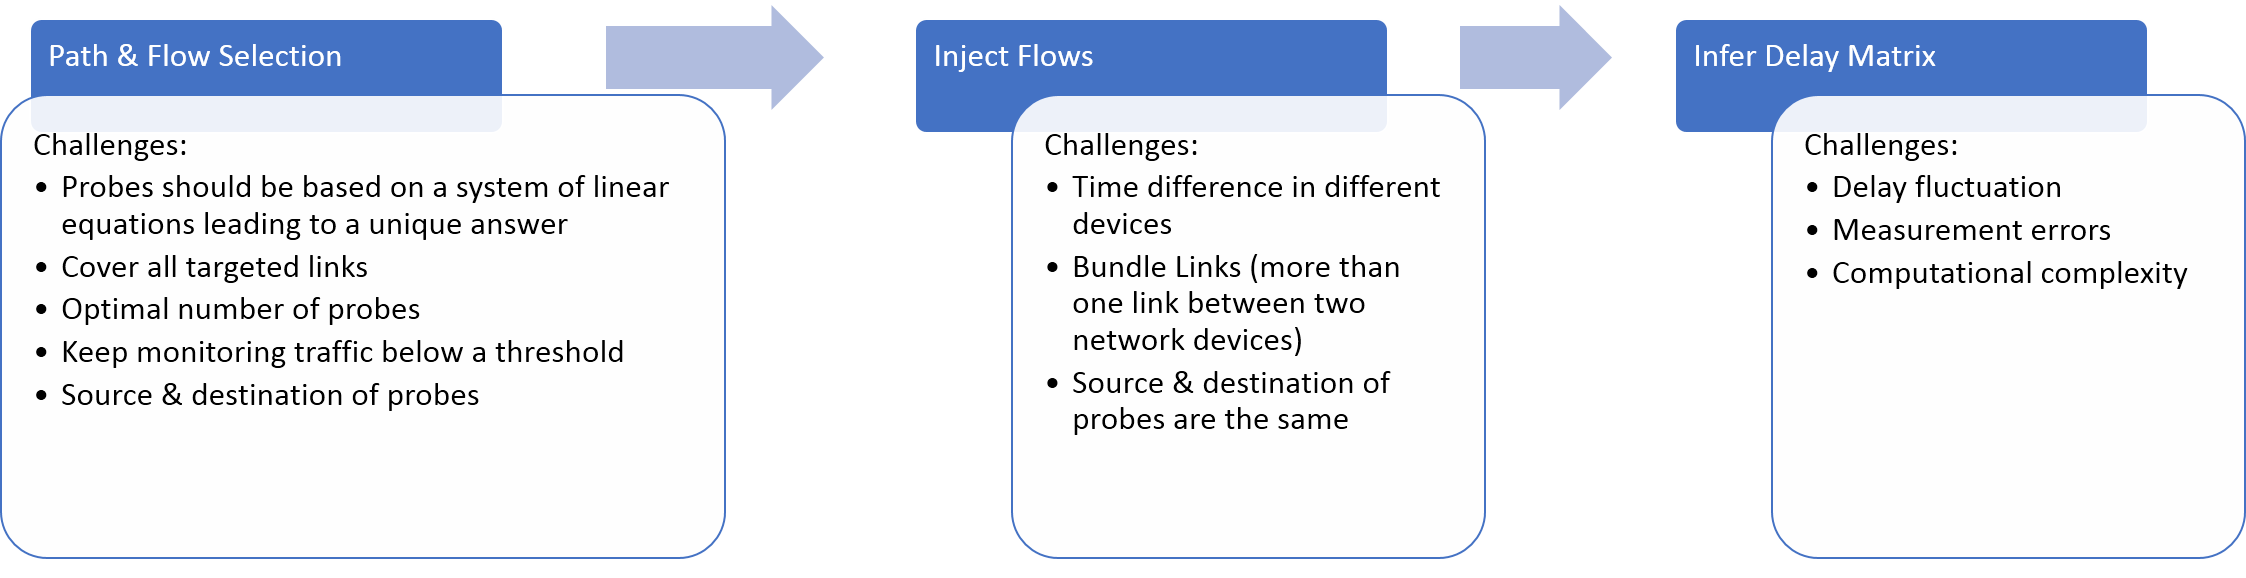
\includegraphics[width=\linewidth]{img/Challenges.png}
    \caption{Steps taken in the proposed solution along with the challenges.}
    \label{fig:challenges}
\end{figure*}
The first step, called \textit{Path $\&$ Flow Selection}, is to define the flows, i.e., specifying the source, destination, and selected hobs (links) throughout the network. This step is the most difficult one, including several challenges. The main challenge is that the assignment of resources (selecting paths for flows) should end up to a system of linear equations (or linear system) with a unique solution. Linear system is a collection of linear equations involving the same set of variables. The equations of a linear system should be independent meaning that none of the equations should be derived algebraically from the others. When the equations are independent, each equation contains new information about the variables, and removing any of the equations increases the size of the solution set. For linear equations, logical independence is the same as linear independence. Fig.~\ref{fig:linear_systems_dependant} shows a sample where the equations are dependant in a 3D environment.
\begin{figure}
    \centering
    \begin{subfigure}{0.49\columnwidth}
          \centering
          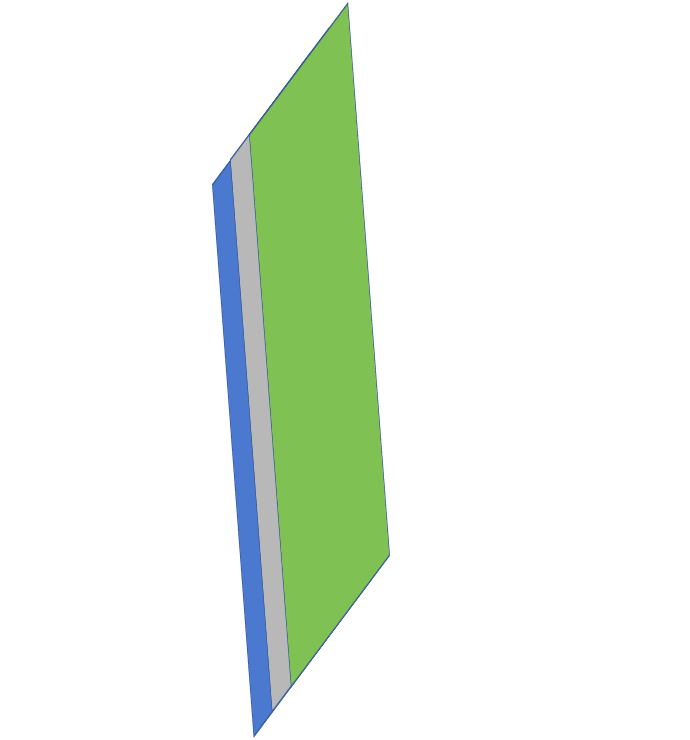
\includegraphics[width=\columnwidth]{img/Dependent3D1.png}
          \caption{Dependent}
          \label{fig:linear_systems_dependant}
    \end{subfigure}
    \begin{subfigure}{0.49\columnwidth}
          \centering
          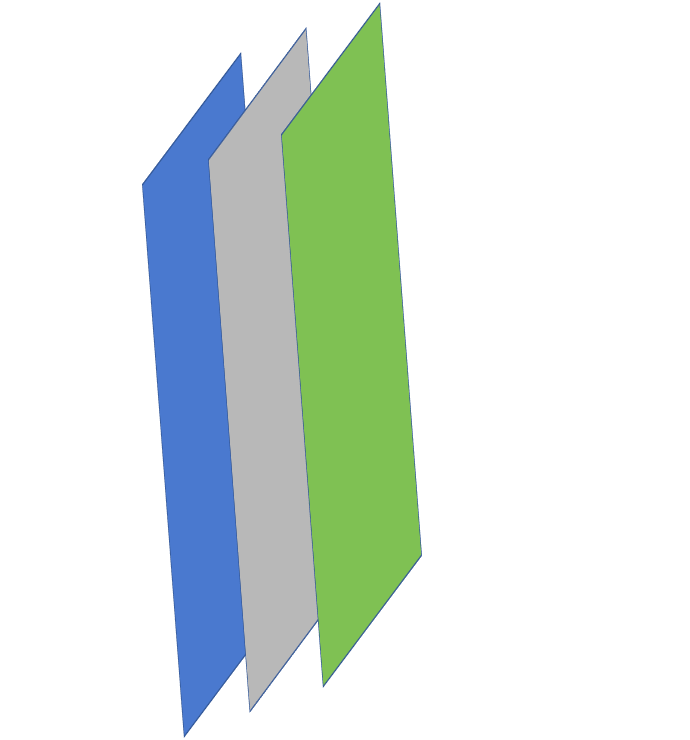
\includegraphics[width=\columnwidth]{img/Inconsistent3D1.png}
          \caption{Inconsistent}
          \label{fig:linear_systems_inconsistent1}
    \end{subfigure}
    % \begin{subfigure}{0.49\columnwidth}
    %       \centering
    %       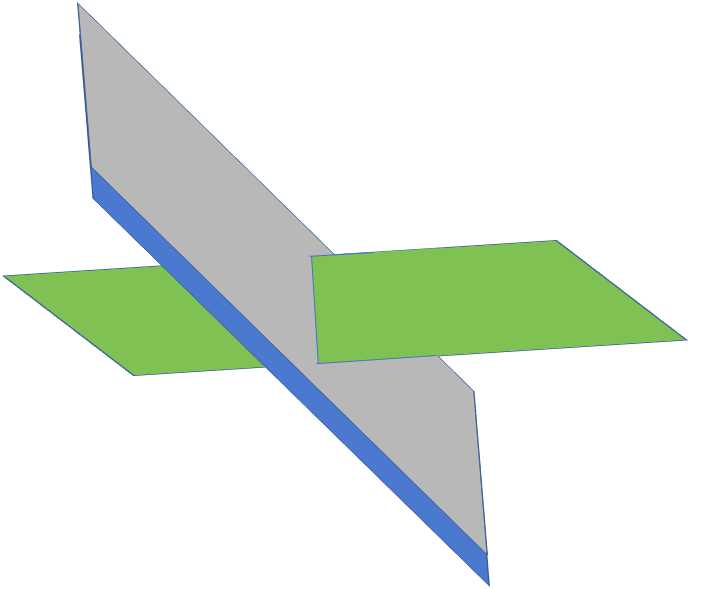
\includegraphics[width=\columnwidth]{img/Dependent3D2.png}
    %       \caption{Dependent}
    %       \label{fig:linear_systems_dependant2}
    % \end{subfigure}
    \begin{subfigure}{0.49\columnwidth}
          \centering
          
\includegraphics[width=\columnwidth]{img/Inconsistent3D2.png}
          \caption{Inconsistent}
          \label{fig:linear_systems_inconsistent2}
    \end{subfigure}
    %\begin{subfigure}{0.49\columnwidth}
    %      \centering
    %      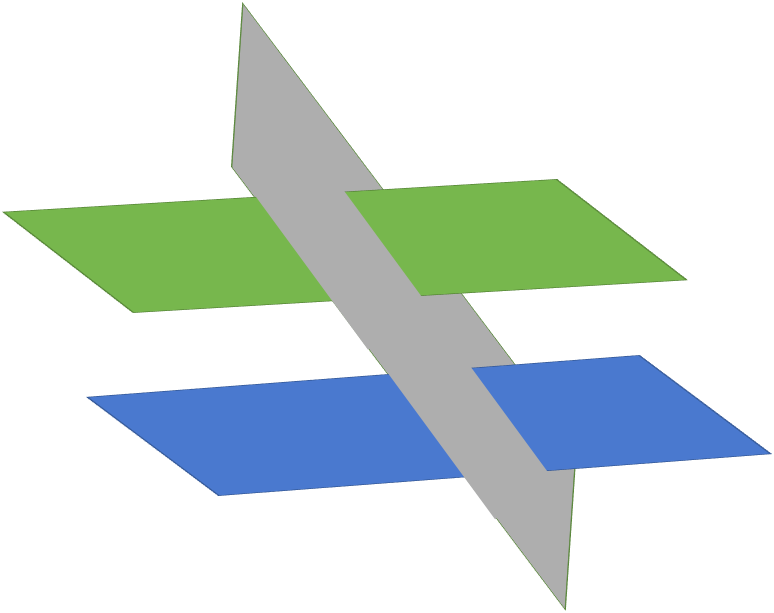
\includegraphics[width=\columnwidth]{img/Inconsistent3D3.png}
    %      \caption{Inconsistent}
    %      \label{fig:linear_systems_inconsistent3}
    %\end{subfigure}
    \begin{subfigure}{0.49\columnwidth}
          \centering
          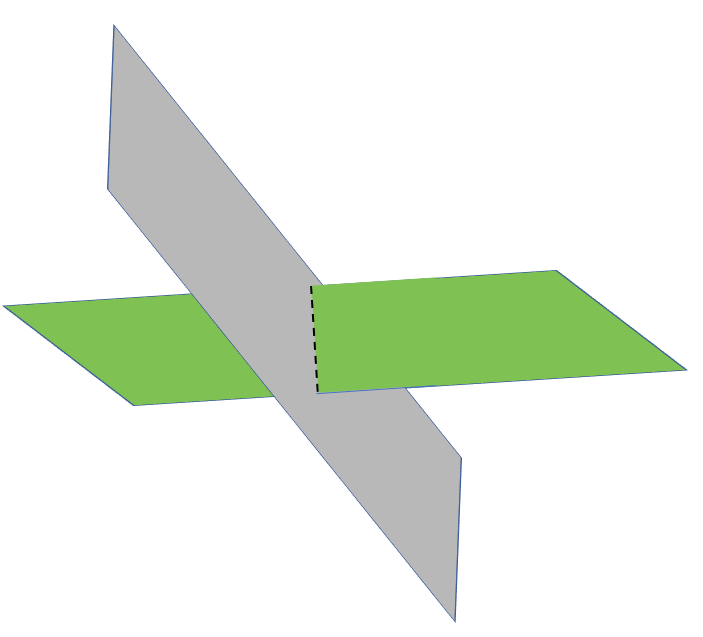
\includegraphics[width=\columnwidth]{img/Many_answer.png}
          \caption{Many Answers}
          \label{fig:linear_systems_many_answers}
    \end{subfigure}
    %\centering
    %\includegraphics{}
    \caption{Improper Linear Systems}
    \label{fig:linear_systems}
\end{figure}
Another mandatory feature of the seeking linear system is consistency. A linear system is consistent if it has a solution, and otherwise, it is said to be inconsistent. When the system is inconsistent, it is possible to derive a contradiction from the equations, that may always be rewritten as the statement 0 = 1. Fig.s~\ref{fig:linear_systems_inconsistent1}~and~\ref{fig:linear_systems_inconsistent2} are examples of inconsistency in linear equations. 

The desired linear system not only should be independent and consistent but also it should lead to one unique answer. For instance, the equations depicted in Fig.~\ref{fig:linear_systems_many_answers} are consistent and independent but leading to many possible answers. An example of a proper system of equations is illustrated in Fig.~\ref{fig:linear_system_perfect}, where solving the system leads to a unique answer.
\begin{figure}
    \centering
    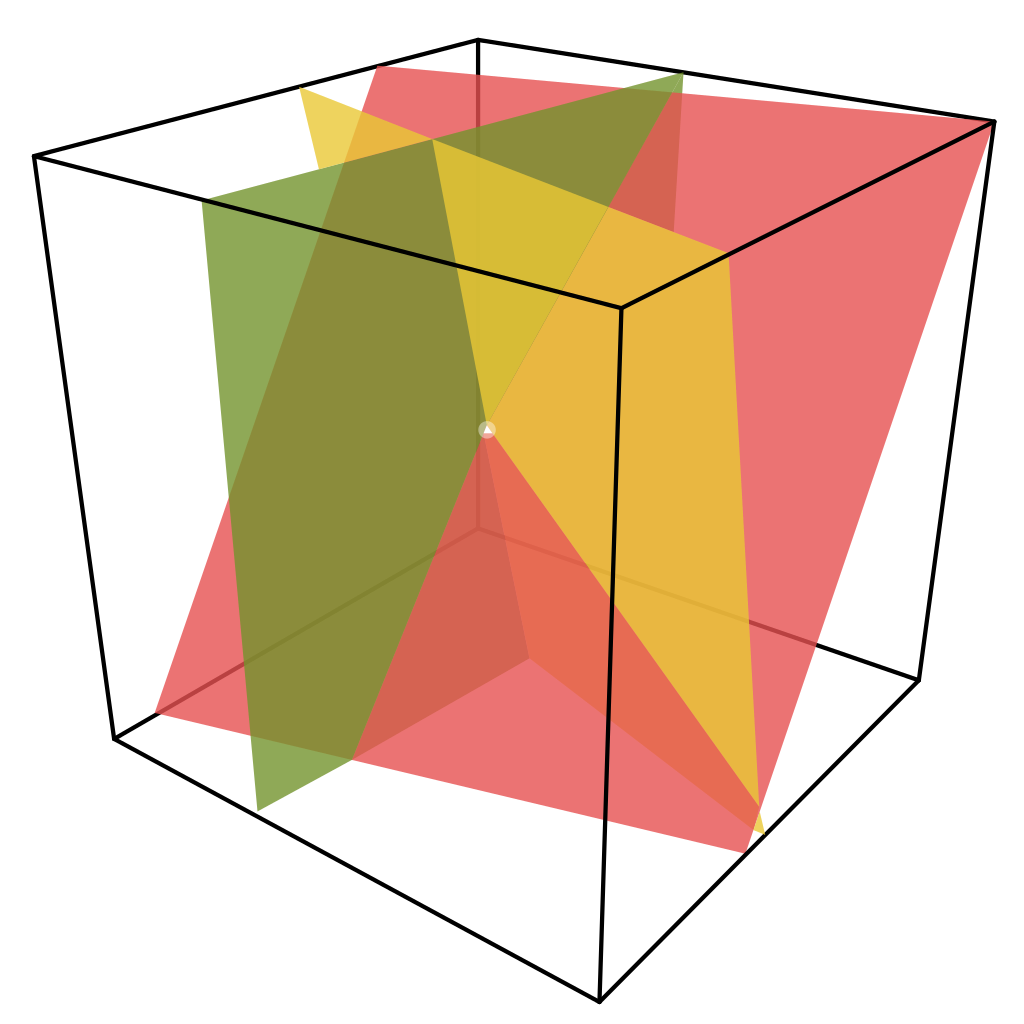
\includegraphics[width=0.49\columnwidth]{img/perfectsolution.png}
    \caption{A proper system of linear equation with one unique answer.}
    \label{fig:linear_system_perfect}
\end{figure}
Another challenge of \textit{path $\&$ flow selection} is to cover all targeted links meaning that all those links should appear in the linear system. In this way, increasing the length of the path each flow take increases the impact measurement error while decreasing the length of the tours increases the number of required flows. On the other hand, the number of flows should stay in a safe zone since decreasing the number of flows may results in a linear system with many possible answers while increasing the number of flows could end-up with too much monitoring traffic or an inconsistent linear system (due to measurement error). Therefore, the number of flows, their source~$\&$~destination, and the way they tour the network have a direct impact on the monitoring overhead.

The second step in the proposed solution is to inject the flows into the network in order to measure their end-to-end delay (called \textit{Inject flows} in Fig.~\ref{fig:challenges}). The main challenge of this part is to handle the time difference of monitoring devices. The error-tolerance of delay-measurement needs to be in a safe zone which is beyond the adjustment accuracy of computer devices. In another word, a computer clock can be thrown off by many factors, including network jitter, delays introduced by software, and even the environmental conditions in which the computer is operating. This means that network delay has an impact on the time accuracy in monitoring devices, therefore, if the source and destination of a flow be two different entities then the one-way delay is not accurately computable due to time difference of source and destination. On the other hand, if delay measurement takes place on a round-trip basis, then the difference of queuing delay over ingress and egress links would be ignored. Meaning that using a round trip measurement ignores some parts of the information. Considering all in mind, the applicable way of measuring one-way delay based on the analysis of flows' end-to-end delay is to set the source and destination to one node. This assumption brings up some implementation issues which is handled in our developed code (all codes are open access and could be reached out in~\cite{monitoringCodeOurImplementation}).

The last step in the proposed solution is to infer the matrix of delay using the information gathered in the previous step. The main challenge, here, is the link-delay-fluctuation and measurement-errors which may cause an inconsistency in the linear system. Obviously, the computational complexity of this part is very important as this part is running with a period manner (but step one is a one-time task which could be done offline). In the following, the mathematical formulation and the meta-heuristic algorithm proposed for \textit{Path $\&$ flow Selection} are described in sec.s~\ref{subsec:mathematical_formulation}~and~\ref{subsec:heuristic_alg}. The meta-heuristic algorithm proposed for inferring the delay matrix is discussed in sec.~\ref{subsec:pso}.

\subsection{Proposed Architecture}
\begin{figure}
    \centering
    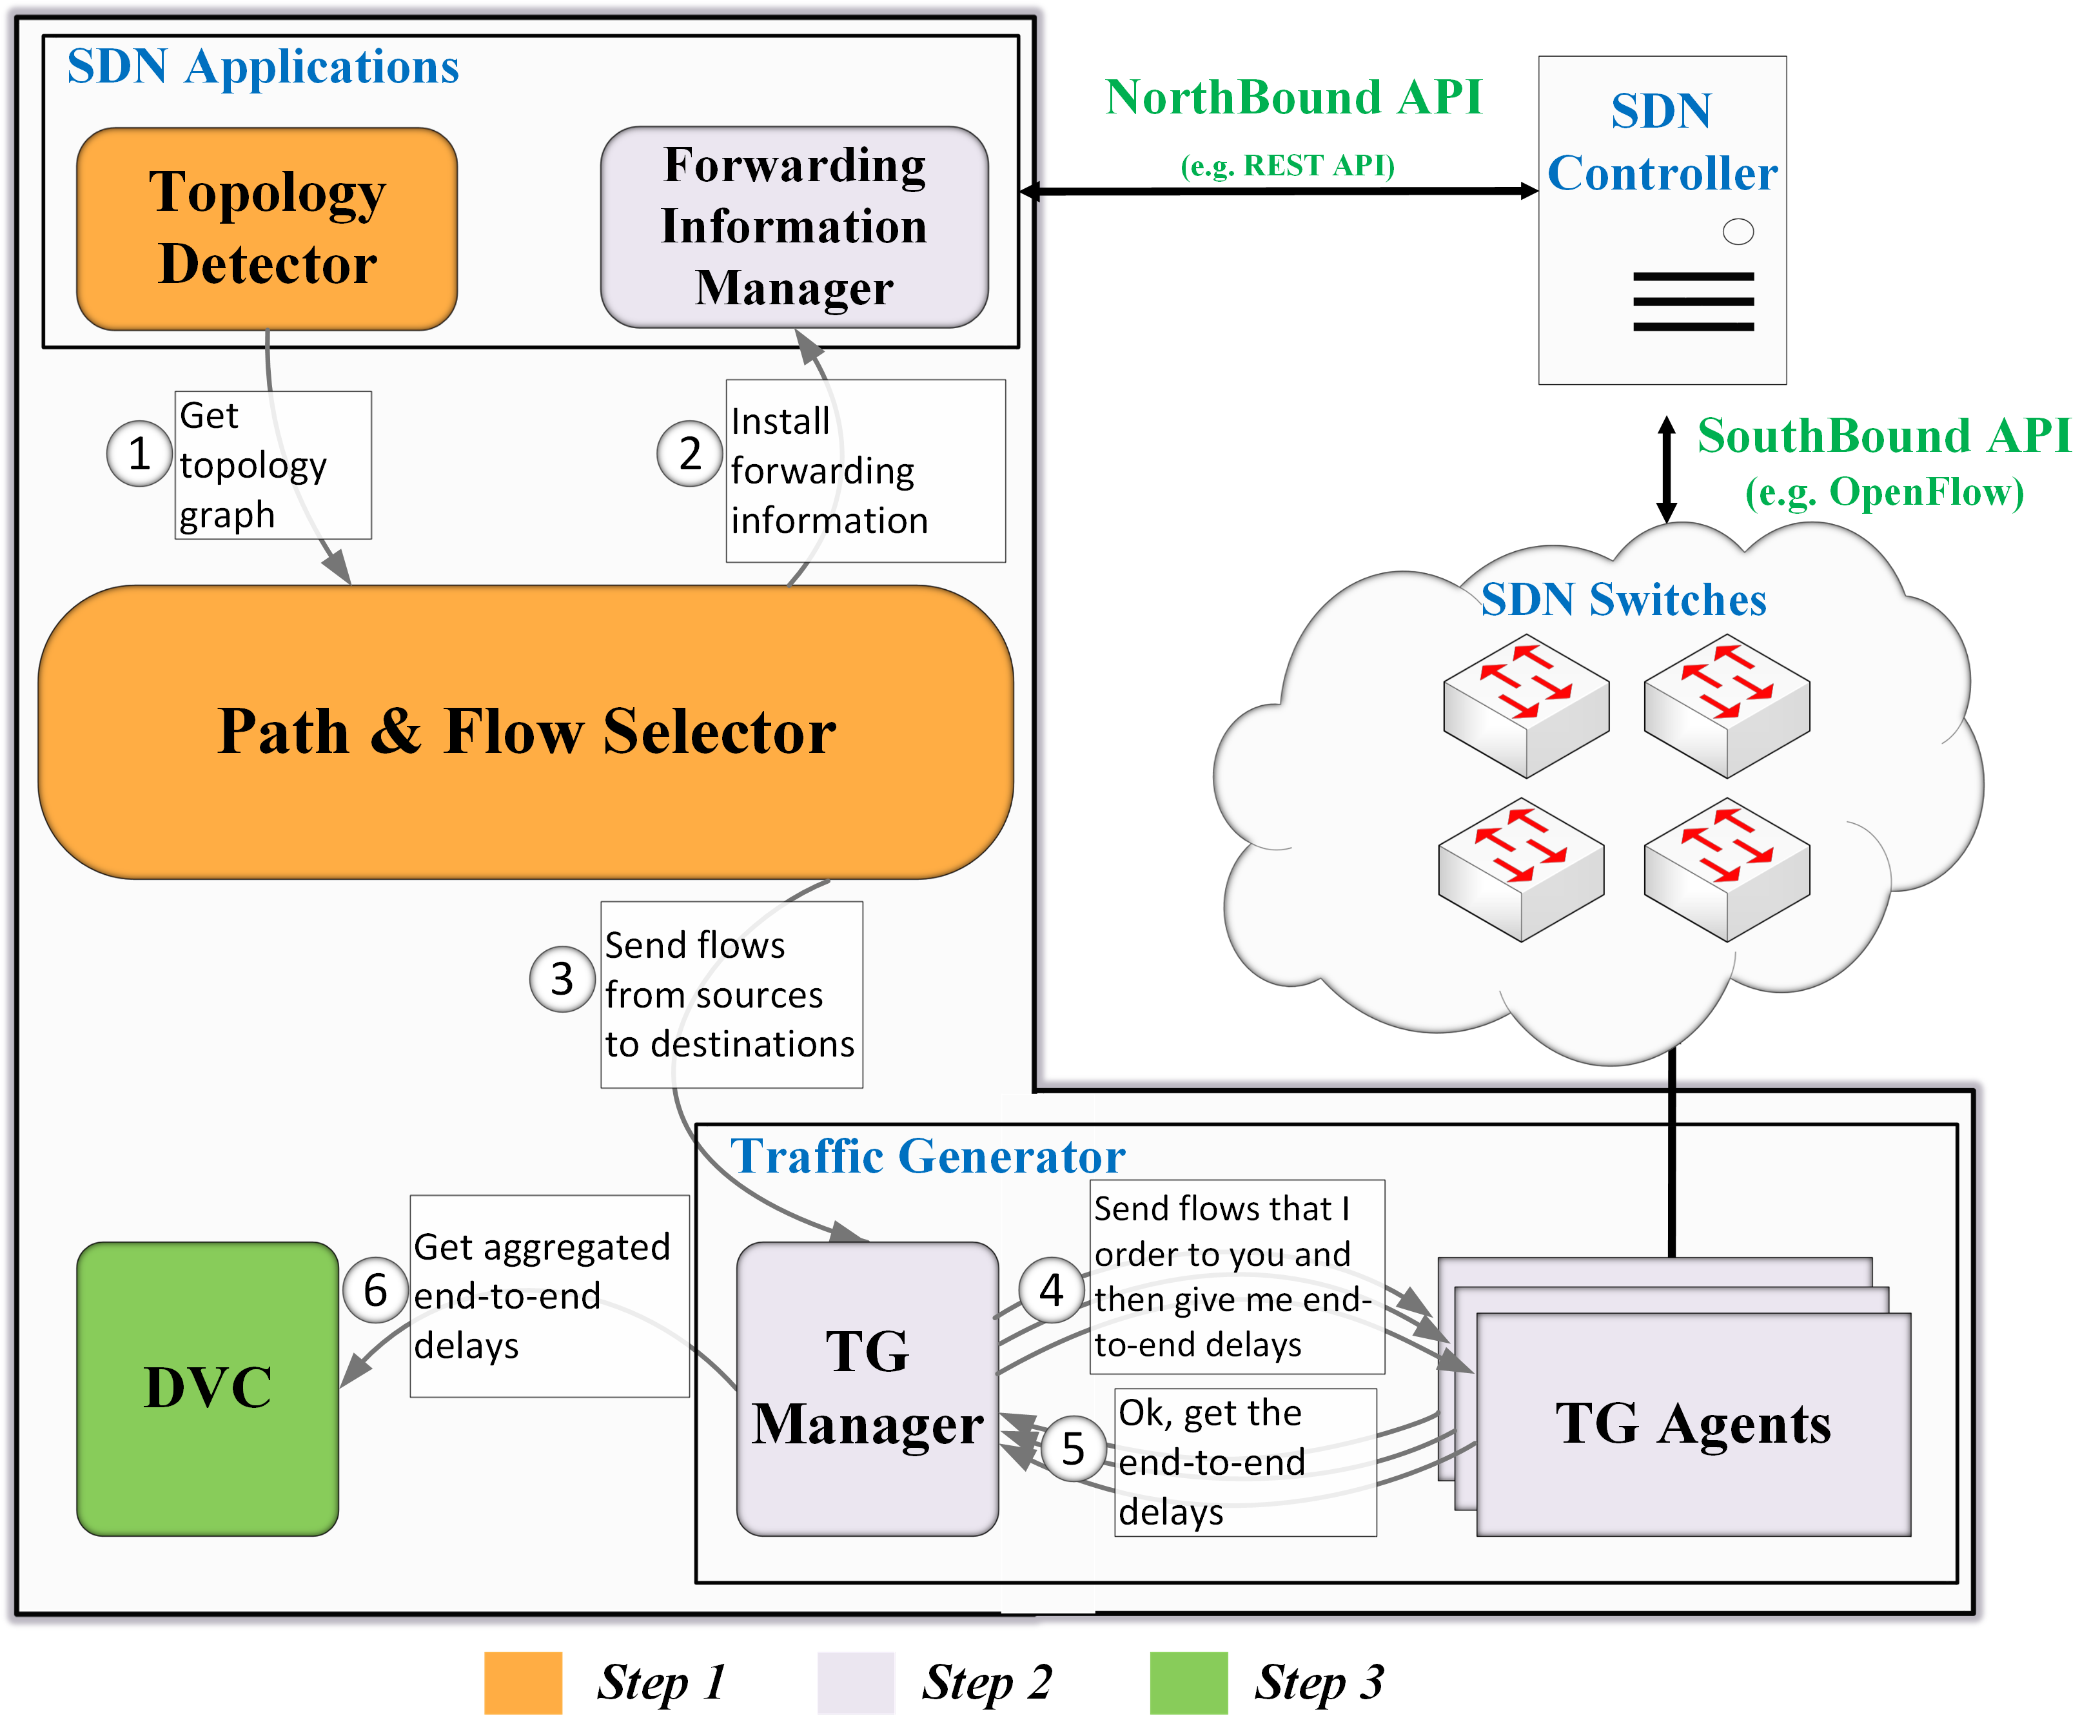
\includegraphics[width=0.49\columnwidth]{img/architecture.png}
    \caption{The proposed architecture.}
    \label{fig:architecture}
\end{figure}
\subsection{Mathematical Formulation of Path $\&$ Flow Selection}\label{subsec:mathematical_formulation}
We consider an SDN-based network in which networking devices are programmed using a southbound protocol (e.g., reference~\cite{ventre2018sdn}). There are a few number of hosts where the monitoring flows origins from. For every monitoring flow, the controller should select a source, destination, and set of links through source to the destination. The length of the selected path for each flow should be less than a predefined threshold. All targeted links should be passed by at least $m$ flows and the source and destination of flows may be the same. We assume a network with $N$ SDN-enabled switches. The network topology is represented with a matrix $B^{\max}_{N\times N}$, where the capacity of the link from the switch $i$ to the switch $j$ is stored in $b_{(i,j)}$. Similarly, $D_{N\times N}$ denotes the link delay, where $d_{(i,j)}$ stores the delay of the link from the switch $i$ to the switch $j$. The number of Monitoring flows in the network is denoted with $F$ and the maximum length of paths assigned is limited by $L^t$. Table~\ref{tab:notation} provides the symbols used though this paper along with a brief description.
\begin{table}[t]
	\caption{Main Notation.}\label{tab:notation}
	\centering
	%	\begin{center}\small
	\resizebox{\columnwidth}{!}{%
	%\tiny
	\begin{tabular}{|c||l|l|} 
		\hline
		& \textbf{Symbol} & \textbf{Description}\\
		\hline\hline
		\multirow{13}{0.1cm}{\begin{sideways}\textbf{Parameters}\end{sideways}} 
		& $E$ & Number of links  \\\cline{2-3}
		& $N$ & Number of monitoring nodes \\\cline{2-3}
		& $\mathcal{N}$ & Set of monitoring nodes \\\cline{2-3}
        & $F$ & Number of monitoring flows \\\cline{2-3}
        & $\mathcal{F}$ & Set of monitoring flows \\\cline{2-3}
		& $B^{\max}_{(i,j)}$ & Matrix of link capacity\\ \cline{2-3}
	    & $D^{\max}_{f}$ & Maximum tolerable propagation \\ \cline{2-3}
	    & $q$ & Average rate of a monitoring flow  \\\cline{2-3}
		& $s^{f}$ & Vector of source switch\\\cline{2-3}
		& $d^{f}$ & Vector of destination switch\\\cline{2-3}
		& $x$ & Min number of monitoring flows on a link\\\cline{2-3}
		& $U$ & Sufficiently big number\\\cline{2-3}
		& $l$ & Max acceptable length for a monitoring flow\\\cline{2-3}
		& $A_{(i,j)}$ & Matrix of adjacency (link from switch i to j)\\ \hline\hline
		\multirow{7}{0.1cm}{\begin{sideways}\textbf{Variable}\end{sideways}}
		& $D_{(i,j)}$ & Links delay\\\cline{2-3}
		& ${\mu}$ & Monitoring traffic to total bandwidth ratio \\ \cline{2-3}
		& $R_{(i,j)}^f$ & Routing matrix \\\cline{2-3} 
		& $T^{(f,f')}$ & Intermediate variable (description in text) \\\cline{2-3} & $Y^{(f,f')}$ & Binary intermediate variable (description in text) \\\cline{2-3}
		& $P_{(i,j)}^f$ & Ordering matrix \\ \hline
    	\end{tabular}}
    	%	\end{center}
    \end{table}
In order to simplify the understanding of the notation, a sample of the proposed notation is presented in the following lines. A network topology with five routing devices can be represented with a $5\times5$ matrix as following:
\[B^{\max}=
  \begin{bmatrix}
    0 & b_{(1,2)} & b_{(1,3)} & 0 & 0\\
    b_{(2,1)} & 0 & 0 & b_{(2,4)} & 0\\
    b_{(3,1)} & 0 & 0 & 0 & b_{(3,5)}\\
    0 & b_{(4,2)} & 0 & 0 & b_{(4,5)}\\
    0 & 0 & b_{(5,3)} & b_{(5,4)} & 0
  \end{bmatrix}\]
\[D=
  \begin{bmatrix}
    \infty & d_{(1,2)} & d_{(1,3)} & \infty & \infty\\
    d_{(2,1)} & \infty & \infty & d_{(2,4)} & \infty\\
    d_{(3,1)} & \infty & \infty & \infty & d_{(3,5)}\\
    \infty & d_{(4,2)} & \infty & \infty & d_{(4,5)}\\
    \infty & \infty & d_{(5,3)} & d_{(5,4)} & \infty
  \end{bmatrix}\]
  
The source and destination of flows are determined by the vectors $s^f$ and $d^f$ determine, respectively. In the proposed solution source and destination of a flow can be the same. Clearly this ends up to a loop in the routing path which is handled in our implementation. Except loops caused by equal source and destination, the other types of loops are not allowed (due to implementation limits). Matrix $A_{(i,j)}$ denotes whether a link from switch $i$ to switch $j$ exists or not. If there is a link then its value is 1 otherwise, 0. $x^t$: In each time slot, exactly $x^t$ monitoring flows travel through the link $(i,j)$. Matrices $R^f_{(i,j)}$ and $P^f_{(i,j)}$ denote the path selected for every monitoring flows. $R^f_{(i,j)}$, the main output of this formulation, shows the steps taken from source to destination without specifying the order. As an example, let the source and destination of flow~1 be node one and node five respectively. 
\[R^1=
  \begin{bmatrix}
    0 & 1 & 0 & 0 & 0\\
    0 & 0 & 0 & 1 & 0\\
    0 & 0 & 0 & 0 & 0\\
    0 & 0 & 0 & 0 & 1\\
    0 & 0 & 0 & 0 & 0
  \end{bmatrix}\]
This means that the flow~1 starts from node one and directly goes to node two ($R^1_{(1,2)}=1$). Then the flows moves out to node four (since $R^1_{(2,4)}$ is one) and finally leave node four toward node five ($R^1_{(4,5)}=1$). Similarly, $P^f_{(i,j)}$ is an intermediate variable showing the selected routing for every monitoring flow considering the ordering of links traversed. Therefore, matrix $P$ for the above mentioned flow is as following:
\[P^1=
  \begin{bmatrix}
    0 & 1 & 0 & 0 & 0\\
    0 & 0 & 0 & 2 & 0\\
    0 & 0 & 0 & 0 & 0\\
    0 & 0 & 0 & 0 & 3\\
    0 & 0 & 0 & 0 & 0
  \end{bmatrix}\]
The mathematical formulation is provided in the following lines. The objective function is to minimize the monitoring overhead by reducing the maximum ratio of monitoring traffic to link capacity.
\begin{align}
    & \min{\mu}
\end{align}

Eq.~\ref{eq:use_existing_links} is used to ensure the links through a path do exists. In other words, flows are forced to use only existing links and do not jump from a router to another one if there is no direct link between them. To this end, the elements of routing matrix $R$ should always be less than or equal to corresponding elements in adjacency matrix $A$.
\begin{align}
    & R_{(i,j)}^f \leq A_{(i,j)}, \forall i, j \in \mathcal{N}, \forall f \in \mathcal{F} \label{eq:use_existing_links}
\end{align}

End-to-end delay may be undergone changes by different transient factors, therefore, to keep the measurement accuracy acceptable, it's better to use more than one flow to infer a link's delay. This means that having more than one flows traversing a link is desirable. Eq.~\ref{eq:flows_per_link} ensures that at least $x^t$ monitoring flows traverse every link. The appearance of adjacency matrix $A$ in the right side of Eq.~\ref{eq:flows_per_link} prevents the algorithm from using links that does not exists.
\begin{align}
    & \sum_{f=1}^{F}{R_{(i,j)}^{f}}\geq x*A_{(i,j)},   \forall i,j \in \mathcal{N} \label{eq:flows_per_link}
\end{align}

The net flow entering a node should be zero, except for the source, which "produces" flow, and the sink/destination, which "consumes" flow. This is usually referred to as "flow conservation constraints". In our mathematical formulation, the flow conservation concept is algebraically implemented in  Eq.~\ref{eq:flow_conservation}. However, here there is a small difference with common flow conservation constraints. In the proposed solution, it is possible to have a node as both source and destination of a flow. But due to challenges for routing in existence of loop, this case is usually unacceptable for most of routing algorithms, i.e., it is not considered in common flow conservation constraints. Therefore, the case where source and destination are the same is excepted from Eq.~\ref{eq:flow_conservation}. We then add a new constraint to handle this exception. Beside, practical solution to tackle the existence of loop for implementation step is discussed in the remainder of this paper.
\begin{align} \label{eq:flow_conservation}
    & \sum_{j=1}^N{\sum_{f=1}^F{R_{(i,j)}^{f}}}+\sum_{f=1}^F{\sum_{j=1}^N{R_{(i,j)}^{f}}}=\\\nonumber
    &~~~~~~~~~~~~~~~~~ \begin{cases}
                     1 & i=s^f~~~~ \And s^f\neq d^f\\
                    -1 & i=d^f~~~~ \And s^f\neq d^f\\
                     0 & i\neq s^f,d^f \And s^f\neq d^f\\
                    \end{cases},  \forall i \in \mathcal{N}
\end{align}

Eq.~\ref{eq:flow_conservation_replacement} substitutes the flow conservation constraint (Eq.~\ref{eq:flow_conservation}) when the source and destination of a flow are the same. In this case, the incoming and outgoing of every node should be zero, regardless of being a source, destination, middle node, or not traversed node.
\begin{align}
    & \sum_{j=1}^N{\sum_{f=1}^F{R_{(i,j)}^{f}}}+\sum_{f=1}^F{\sum_{j=1}^N{R_{(i,j)}^{f}}}= 0,~~~ s^f=d^f, \forall i \in \mathcal{N} \label{eq:flow_conservation_replacement} 
\end{align}

One of the most important criteria that should be met is keeping the monitoring overhead as low as possible. There are several metrics to measure the overhead including the amount of monitoring traffic and the number of monitoring rules on routing devices. Eq.~\ref{eq:monitoring_overhead} ensures the monitoring flows use at most $\mu^t$ percent of link bandwidth.
\begin{align}\label{eq:monitoring_overhead}
    & \sum_{f=1}^F{R_{(i,j)}^{f}}\times q\leq \mu\times B_{(i,j)},   \forall i,j \in \mathcal{N}
\end{align}

There are two reasons for a loop to exists in a computer network: to meet a node twice or due to an error in the routing algorithm. If the loop is formed by an error in the routing algorithm then the path to a particular destination forms an infinite loop. This means that the nodes keep forwarding the packet to each other until an external reason (e.g., packet timer) intervene the routing. In our formulation, to prevent an unwanted loop creation, Eq.~\ref{eq:loop} is added. This equation prevents a loop in routing unless the source and destination are the same (this is a type of loop that does not make any problem).
\begin{align}\label{eq:loop}
    & \sum_{j=1}^N{R_{(i,j)}^{f}}\leq 1
\end{align}

Due to the dynamic nature of link delay, it is desired to have an upper bound on the number of links a monitoring flow traverse. To this end, Eq.~\ref{eq:flow_length} keeps the length of monitoring routes less than a predefined value.
\begin{align} \label{eq:flow_length}
    & \sum_{i=1}^N{\sum_{j=1}^N{R_{(i,j)}^{f}}}\leq l,     \forall f\in \mathcal{F}
\end{align}

Eq.~\eqref{eq:R_Zero} hints that if the value of matrix $A_{(i,j)}^f$ is zero, then $P^f_{(i,j)}$ becomes zero. It also indicates that the value of the ordering matrix should be higher or equal to the rerouting matrix.
\begin{align} \label{eq:R_Zero}
    & P_{(i,j)}^{f}\leq l\times R^f_{(i,j)},     \forall i,j \in \mathcal{N}, \forall f\in \mathcal{F}
\end{align}

The elements of ordering matrix specify the steps through the way from source to destination. Therefore, if the step number assigned to the flow entering a node $n$ is $X$ then step number assigned to that flow leaving node n should be $X+1$. This means that ordering matrix should always be equal to or greater than routing matrix. Briefly, the step number in ordering matrix should always increase by one after leaving a node. This criteria is guaranteed via Eq.~\ref{eq:step_P} in our formulation.
\begin{align} \label{eq:step_P}
    & \sum_{j=1}^N{P_{(i,j)}^{f}} = \sum_{j=1}^N{\left(P_{(j,i)}^f+R_{(j,i)}^f\right)}, \\\nonumber
    &~~~~~~~~~~~~(i\neq s^f ~or~ i\neq d^f), \forall i\in \mathcal{N}, \forall f\in \mathcal{F}
\end{align}

In our formulation, in order to deal with the time inconsistency between different nodes (in microsecond granularity), the source and destination of a flow may be the same. The following equations ensure that monitoring flows leave the source node and enter the destination node. This is because if the source and destination are the same the flow has reached the destination without leaving it. In other words, without the following equations, some flows will not leave the source.
\begin{align}
    & \sum_{j=1}^N{R^f_{(s^f,j)}}=1, \forall f\in \mathcal{F}\\
    & \sum_{i=1}^N{R^f_{(i,d^f)}}=1, \forall f\in \mathcal{F}
\end{align}

A solution for the proposed mathematical formulation may end up with similar routes assigned to flows with similar pairs of source $\&$ destination. Meaning that some flows are a duplication of others. Duplicating a flow (having two flows traversing similar nodes) do not add any extra information regarding the links' delay. However, this adds a new limit on the diversity of source $\&$ destination because completely different pairs of source $\&$ destination should be used for flows. Consequently, the number of required monitoring nodes to measure the delay of a set of links increases. To avoid this, the formulation should take diversity in routes as a criterion for flows with similar pairs of source $\&$ destination.
\begin{align}\label{eq:T}
    & T^{(f,f')} = \sum_{i=1}^N{\sum_{j=1}^N{\left(((N+1)\times i+j)\times R_{(i,j)}^f\right)}} - \nonumber\\ 
    &~~~~~\sum_{i=1}^N{\sum_{j=1}^N{\left(((N+1)\times i+j)\times R_{(i,j)}^{f'}\right)}}
\end{align}    
In order to simplify the formulation, intermediate variable $T^{(f,f')}$ is defined in Eq.~\ref{eq:T}. This variable compares the routes assigned to flows $f$ and $f'$ and computes a value for their similarity based on the equation provided in Eq.~\ref{eq:T}. 
\begin{align}
    & T^{(f,f')} \leq  Y^{(f,f')}\times U, \forall f,f'\in \mathcal{F}, f<f'\\
    & T^{(f,f')} \geq  -Y^{(f,f')}\times U, \forall f,f'\in \mathcal{F}, f<f'\\
    & T^{(f,f')} \geq 1- Y^{(f,f')}\times (N+1)\times U, \forall f,f'\in \mathcal{F}, f<f'
\end{align}
$Y$ is another intermediate variable used along with $T$ to ensure there is no repeated path. $Y$ is a binary variable and it does not carry a meaningful value. This variable ensures the value assigned to comparison of $f$ and $f'$ stay in the acceptable area.

\subsection{Heuristic Algorithm for Path $\&$ Flow Selection}\label{subsec:heuristic_alg}
The mathematical formulation discussed in the previous section is computationally complex to be solved even for small-size networks. Therefore, a heuristic algorithm is proposed in Alg.~\ref{alg:HILP} to solve the corresponding optimization problem in a rational time. The heuristic algorithm proposed for Path $\And$ Flow Selection is called \textit{PFS}. The algorithm is designed in a recursive and greedy manner with a sufficiently low computational complexity.

\begin{algorithm}[!htbp]
	\caption{Pseudo-Code of Path $\&$ Flow Selection (\textit{PFS})}
	\label{alg:HILP}
	%\normalsize
	\small
	\allowdisplaybreaks
	\begin{algorithmic}[1]
	   % \setstretch{1.5}
    	%\break
    	\INPUT{$<$\textit{Topo}, \textit{AL}, \textit{TL}$>$}
    	\LineComment{Topo: Network topology}
    	\LineComment{AL: Allowed lengths for monitoring flows}
    	\Statex{\texttt{TL: Targeted links (links to monitor)}}
    	\OUTPUT{$<$\textit{ULSF},\:\textit{SRSF}$>$}
    	\State{\textit{ULSF}=$\emptyset$}
    	\LineComment{~~ULSF: Used Links So Far}
    	\State{\textit{SRSF}=$\emptyset$}
    	\LineComment{~~SRSF: Selected Routes So Far}
    	\State{\textit{PS} = Extract\_List\_of\_Possible\_Sources(Topo)}
    	\LineComment{~~PS: Possible sources}
    	\State{\textit{A}, \textit{B} = Convert\_Topo\_to\_Graph(\textit{Topo})}
    	\LineComment{~~Mapping IP/MAC to numbers and demonstr-}
    	\LineComment{~~ating as matrix}
    	\LineComment{~~A: Adjacency matrix, B: Capacity matrix}
    	\For{\textit{length} $\in$ \textit{AL}}
        	\For{\textit{src} $\in$ \textit{PS}}
        	    \State{Find\_Routes(\textit{src, length, A, B, *ULSF, *SRSF, TL})}
        	    \LineComment{~~A recursive function calculating }
        	    \LineComment{~~the routes and deciding on the }
        	    \LineComment{~~number of required monitoring flows}
        	   % \State{UL, SR = Find\_Routes(src, length, A, B, ULSF, SRSF)}
        	   % \LineComment{~~UL: Used Links, SR: Selected Routes}
        	\EndFor
    	\EndFor\\
	    \Return{$<$\textit{ULSF,\:SRSF}$>$}
	\end{algorithmic}
\end{algorithm}

\textit{PFS} takes the network topology, targeted links (links to be monitored), and allowed lengths for monitoring flows and makes a decision on the number of required flows. Thereafter, the algorithm computes the routes for every monitoring flows in a way that all targeted links be traversed by at least $x$ flows. In the first 4 lines of Alg.~\ref{alg:HILP}, the preliminaries are done which includes finding the possible sources for the monitoring flows as well as converting the network topology into adjacency and bandwidth matrices. After that, for each possible pair of length of flow and source node \textit{PFS} generate a couple of flows. This will continue until all possible flows are added, however, one may decide to continue the process until all required links are included in the routes. 

\begin{algorithm}[!htbp]
	\caption{Pseudo-Code of Find\_Routes Function}
	\label{alg:FindRoutes}
	%\normalsize
	\small
	\allowdisplaybreaks
	\begin{algorithmic}[1]
	   % \setstretch{1.5}
    	%\break 
    	\INPUT{$<$\textit{CN, RH, A, B, ULSF, SRSF, TL, DN=$\emptyset$, SR=$\emptyset$, SN=$\emptyset>$}}
    	\LineComment{CN: Current node, RH: Remaining hops}
    	\LineComment{A: Adjacency matrix, B: Capacity matrix}
    	\LineComment{ULSF: Used Links So Far}
    	\LineComment{SRSF: Selected Routes So Far}
    	\LineComment{DN: Destination node, SR: Selected route}
    	\LineComment{SN: Source node, TL: Targeted links}
    	\OUTPUT{$<>$}
    	\If{\textit{RH}=0}
    	    \If{\textit{CN = DN} $\And$ \textit{SR} $\neq\emptyset$}
    	       \State{Update \textit{ULSF} $\And$ \textit{SRSF} based on \textit{SR} and \textit{TL}}
    	    \EndIf
    	   % \State{\Return{}}
    	\Else
    	    \If{\textit{DN}=$\emptyset$} \textit{DN=CN} \EndIf
    	    \If{\textit{SN}=$\emptyset$} \textit{SN=CN} \EndIf
    	    \For{all nodes \textit{n} connected to \textit{CN}}
    	        \If{\textit{n} $\notin$ \textit{SR} $\And$ no loop in (\textit{SR+n})}
    	            \State{Find\_Routes(\textit{n, RH-1, A, B, ULSF, SRSF, }}
    	            \Statex{~~~~~~~~~~~~~~~~~\textit{DN, SR+n, SN})}
    	        \EndIf
    	    \EndFor
    	\EndIf
	\end{algorithmic}
\end{algorithm}

The pseudo code explained in Alg.~\ref{alg:FindRoutes}, is a recursive approach to find possible monitoring flows which traverse some of the targeted links. The algorithm takes the source, destination, current node, set of targeted links, allowed remained hops (allowed length minus taken hops) as input and returns the set of possible monitoring flows starting from source and ending to destination with specified number of hops.

\subsection{Injection of Flows to the Network (Monitoring Flow Generator)}
In order to inject the monitoring flows into the network, a component called Traffic Generator is defined. This component consists of two main parts: Manager and Agent. The task of the Traffic Generator Manager (TGM) is to communicate directly with the coordinator (which is Path $\&$ Flow Selection algorithm) to report the network topology and receives the list of required monitoring flows. Thereafter, TGM communicates with Traffic Generator Agents (TGAs) and configure them to inject the monitoring flows into the network. Every TGA instance should inject the requested flows and then returns the end-to-end delay assigned to those flows to TGM. 



Our ILP algorithm needs to know the network topology to calculate from which source the probes are sent. This topology can be discovered using the LLDP packets that the Floodlight controller sends to the network switches. It also identifies hosts through ARP broadcast packets. This controller gives us an API that can be used to access topology information such as links, switches and hosts.

We need to generate a variety of traffic to run the ILP algorithm in Coordinator, which is explained \textcolor{red}{in section ()}. By creating this traffic, called a probe, end-to-end delays can be calculated in different paths. Probes can be in two forms. The former are probes that are sent from one host to another, and the second are probes that are transmitted from one host to another. In the following we describe in detail how to produce and direct these two types of probes.

type 1) We want to calculate end-to-end delay from h1 to h2. As you can see in figure (), there are two paths between h1 and h2 that we call theme path a and path b, respectively.
\begin{itemize}
    \item path a: $h1\rightarrow s1\rightarrow s2\rightarrow s4\rightarrow h2$
    \item path b: $h1\rightarrow s1\rightarrow s3\rightarrow s4\rightarrow h2$
\end{itemize}

To be able to detect in s1 switch that the packet sent from h1 must be sent from path a or path b, we need a mechanism to tag the probe packets at the source host.

In this article, we use the type of service field in the IP header to tag probe packets. The tos field is located in the IP layer of the packets and is an 8-bit field, so we can have 256 different tos and assign each tos to a path. In fact, we can have 256 different probes for each pair host (eg h1 and h2).

If we are going to explain this a little deeper, consider that we need to send 2 probes from h1 to h2 and all probes pass through the s1 switch. In this case, we need to install 2 flow entries in s1, for each probe.

Probe 1: flow1: eth_src: h1_mac, eth_dst: h2_mac, ip_tos:1 $\rightarrow$ action: output,2
Probe 1: flow2: eth_src: h2_mac, eth_dst: h1_mac, ip_tos:1 $\rightarrow$ action: output,1

Probe 2: flow1: eth_src: h1_mac, eth_dst: h2_mac, ip_tos:2 $\rightarrow$ action: output,3
Probe 2: flow2: eth_src: h2_mac, eth_dst: h1_mac, ip_tos:2 $\rightarrow$ action: output,1

Now if we send an ICMP probe packet from h1 to h2 and set its ip_tos field to 1, this packet will be sent from path a, and if we put ip_tos to probe 2, that packet will be sent from path b; In fact, we can calculate end-to-end delay in two different paths by sending 2 probes. 

The above example is a probe that is sent from one host to another. Consider the latter. Sometimes we need to send a probe from a host to a switch. Consider Figure ().

We need to send a probe as h1$\rightarrow$ s1$\rightarrow$ s2$\rightarrow$ s3$\rightarrow$ s4$\rightarrow$ s1$\rightarrow$ h1. In h1 we create a probe with the following properties:

h1$\rightarrow$ h helper, ip\_tos: 1

Since the probe is not going to another host, then we need to send the probe from h1 to a hypothetical host that does not exist in the network at all. 

We call this host a helper. So at h1, to generate the probe we need to send it to the helper and we will need to set ip\_tos to tag it. In s1 switch, we install the following flow entry:

eth\_src: h1, eth\_dst: helper, ip\_tos: 1, action: output, 2

In other switches, flow entries are installed in the same way. But the main point is that if we return the same packet produced by h1 to it, can h1 accept it as a return probe? The answer is naturally negative, since h1 waits for the probe to return to him from another host (not himself!). So we need to make a small change during the probe's return to h1. This change occurs in switch s1 (last switch):

eth_src: h1, eth\_dst: helper, ip_tos: 1, actions: output, 2; eth\_src $\rightarrow$ helper_mac; eth\_dst $\rightarrow$ h1_mac;
icmp\_type $\rightarrow$- 0

As you can see, in addition to h1 being defined as a destination, we also need to change icmp\_type to 0. As we know in icmp echo request packet the icmp\_type field is 6 and in icmp echo reply packets the icmp\_type field must be 0.

With the methods outlined above, probes can be sent from one host to another as well as from one host to a switch, and then calculate end-to-end delays in those paths.

For some probes, the delay may be abnormally low or high, we repeat each probe 20 times and then, using a normal distribution, remove RTTs that are $10\%$ higher and $10\%$ lower. We have been. This method will remove invalid data and the remaining average data is prepared for use in the PSO algorithm.

\subsection{Meta-Heuristic Algorithm for Inferring Delay matrix}\label{subsec:pso}
In this subsection, the problem is to take a list of end-to-end delays and routing paths (traversed by each monitoring flow) as input and infer the link delay on targeted links. In fact, the problem is a linear system of equations where the delays of the links are unknowns and the end-to-end delays are fixed values. To solve the aforementioned problem a population swarm optimization (PSO) algorithm is exploited. This meta-heuristic algorithm is called Delay Matrix Inferation (DMI) algorithm. 
\begin{figure}
	\begin{center}
		\begin{tabular}{|c|c|c|c|c|c|c|c|c|c|c|}\hline
			1.2 & 1.0 & 0.5 & 0.8 & 2 & 1.5 & 0.4 & 0.3 & 0.8 & 1.1\\\hline
		\end{tabular}
		\caption{An particle in the proposed PSO algorithm showing the delay of 10 links. In this example, the measurement unit for all values is considered to be millisecond.}
		\label{fig:particle}
	\end{center}%\vspace{-20px}
\end{figure}
In DMI, each particle is a list of delays for targeted links. Let the number of targeted links be 10 (considering each direction as one targeted link), Fig.~\ref{fig:particle} shows a sample particle of the proposed algorithm. The first value in the representation of the particle is 1.2 meaning that the link delay for the first targeted link is 1.2ms (considering milliseconds as the measurement unit).

Alg.~\ref{alg:DMI} shows the pseudo code of DMI. In this algorithm, a random initial population is generated in line 1 and thereafter, the population is enhanced by adding an elite particle. Let \textit{x} be number of particles and \textit{y} the number of targeted links (unknowns). In order to generate the initial population, $x-1$ particles should be generated. Each particle is a list of \textit{y} values showing the delay of one of the targeted links. Initial\_Population function generates $(x-1)\times y$ random values as the first generation of outcomes. LSS function in line 2 of the algorithm, returns the least-squares solution to a linear matrix equation. LSS solves the equation $ax = b$ by computing a vector $x$ that minimizes the squared Euclidean 2-norm $\| b - a x \|^2_2$. The equation may be under-, well-, or over-determined (i.e., the number of linearly independent rows of $a$ can be less than, equal to, or greater than its number of linearly independent columns)\cite{lstsq}. Besides, due to measurement error is linear system of equations may not have a exact solution, therefore, a PSO algorithm is exploited to find the best possible solution.

\begin{algorithm}[!htbp]
	\caption{Pseudo-Code of DMI Function}
	\label{alg:DMI}
	%\normalsize
	\small
	\allowdisplaybreaks
	\begin{algorithmic}[1]
	   % \setstretch{1.5}
    	%\break 
    	\INPUT{$<$\textit{A, SR, EED, TL}$>$}
    	\LineComment{A: Adjacency matrix, SR: Selected route}
    	\LineComment{EED: End-to-End delays, TL: Targeted links}
    	\OUTPUT{$<D>$}
    	\State{\textit{population} = Initial\_Population(\textit{TL})}
    	\LineComment{Generate \textit{x-1} particles. For each particle, generate y random value assigning them as a delay value to every link.}
    	\State{\textit{population} += LSS(\textit{EED, SR})}
    	\LineComment{Add least-squares solution of the linear equations as a particle to the population.}
    	\For{t=1: maximum\_generations}
    	    \For{\textbf{each} particle \textit{p} in \textit{population}}
    	        \State{\textit{fp} = Fitness\_Function(\textit{p})}
    	        \LineComment{Use \textit{p} to solve the linear system} 
    	        \LineComment{and consider the fitness as -error.}
    	        \If{\textit{fp} is better than \textit{fpBest}}
    	            \State{\textit{fbest\_p = fp}}
    	            \State{\textit{best\_p = p}}
    	        \EndIf
    	    \EndFor
    	    \For{\textbf{each} particle \textit{p} in \textit{population}}
    	   		\LineComment{Update velocity}
    	   		\For{$i = 1: y$}
    	   		    \State{Generate two random values $r_1$ and $r_2$}
    	   		    \State{$cognitive=c_1\times r_1\times(best\_p[i]-p[i])$}
    	   		    \LineComment{~$c_1$: Cognitive constant (attraction} 
    	   		    \LineComment{~to best particle vs selfishness)}
    	   		    \State{$social=c_2\times r_2\times(best\_p[i]-p[i])$}
    	   		    \LineComment{~$c_2$: Social constant (attraction to}
    	   		    \LineComment{~social behaviour)}
    	   		    \State{$velocity_{p[i]}=w\times velocity_{p[i]}+cognitive+social$}
    	   		    \LineComment{~$w$: Constant inertia weight (how} 
    	   		    \LineComment{~much to weigh the previous}
    	   		    \LineComment{~velocity)}
    	   		\LineComment{Update position}
    	   		\State{$position_{p[i]}=position_{p[i]}+velocity_{p[i]}$}
    	   		\State{Correct $position_{p[i]}$ by keeping it in boundaries}
    	   		\EndFor
    	    \EndFor
    	    \If{fbest\_p is zero}\State{\Return{best\_p}}\EndIf
    	    \If{best\_p has no improvement during \textit{m} generations}
    	        \State{\textit{population} = Mutation(\textit{population})}
    	        \LineComment{~Randomly change some of particles} 
    	        \LineComment{~velocities $\&$ positions}
    	    \EndIf    
    	\EndFor
	\end{algorithmic}
\end{algorithm}

Let maximum\_generations be the maximum number of iteration the particles move they positions. Line 3 makes a loop over actions applied to the population to move into a new generation. Thereafter, for each particle in the population, the fitness is calculated. The error of solving the linear systems using the positions reported in a particle is considered as the negative of fitness for that particle. During the calculation of fitness, the best particle is specified. At this point, the particles start to move around considering several factors: their current position, the position of the best particle, and their velocity. Every particle makes a trade-off between going toward the way it is going and approaching the position of the best particle (lines 12-19). If the best particle does not show any improvement in the fitness over \textit{m} generations, this means that either the population is trapped in a local optimum or the measurement error is too high making the linear systems unsolvable. Therefore, to make sure the population is not trapped in a local optimum a mutation algorithm is considered to free some particles from local optimum. Finally, in order to reduce the execution time when the algorithm has found the desired solution, lines 21-23 are developed which stops the algorithm and returns back the best solution found so far.

\section{Interesting Text}
Today, ten Autonomous Systems (ASes) alone contribute 70$\%$ of the traffic [20], whereas in 2007 it took thousands of ASes to add up to this share [15]. This consolidation of content largely stems from the rise of streaming video, which now constitutes the majority of traffic in North America [23]. This video traffic requires both high throughput and has soft real-time latency demands, where the quality of delivery can impact user experience [6].\cite{schlinker2017engineering}

Most datacenters still use Equal Cost Multi-Path (ECMP), which performs congestion-oblivious hashing of  ows over multiple paths, leading to an uneven distribution of traffic. Alternatives to ECMP come with deployment challenges, as they require either changing the tenant VM network stacks (e.g., MPTCP) or replacing all of the switches (e.g., CONGA)

We can use link delay matrix to do a dynamic and more efficient flowlet routing.

2 hob segment routing is as good as pure segment routing\cite{bhatia2015optimized}

Use this monitoring technique to monitor Virtual Networks. How can cloud operators monitor VNET performance, given black-box tenants? Can physical tools [9, 12, 18] be usefully adapted to virtualized networks?
(2) How accurate are adapted monitors within virtualized envi- ronments? Can they detect customer-impacting faults? Do they exhibit high precision and recall?
(3) Beyond monitoring, how do virtual environments impact fault management? How might we triage which layer of the network is resposible for a fault? How are fault diagnosis, root-causing and mitigation impacted?
[2018-Sigcomm-Cloud Data center ...]

In virtual network monitoring, VNET pingmesh shows the e2e latency so they add the servers latency into consideration. while for system upgrading and stuff like network measuring we just want to know the links and queuing delay of network. Additionally, by them, we cannot undersand the hight latency is caused by servers or network congestion.

Hence the Pingmesh Controller needs to be fault-tolerant and scalable. We use Software Load-Balancer (SLB) [14] to provide fault-tolerance and scalability for the Pingmesh Controller. See [9, 14] for the details of how SLB works. [2015-sigcom-pingmesh]

In this section, we introduce how Pingmesh helps detect switch silent packet drops. When silent packet drops happen, the switches for various reasons do not show information about these packet drops and the switches seem innocent. But applications suffer from increased latency and packet drops. How to quickly identify if an ongoing live-site incident is caused by switch silent packet drops therefore becomes critical. In the past, we have identified two types of switch silent packet drops: packet black-hole and silent random packet drops.

\cite{yaseen2018synchronized} "When monitoring a network, operators rarely have a  ne- grained and complete view of the network’s state. Instead, today’s network monitoring tools generally only measure a single device or path at a time; whole-network metrics are a composition of these independent measurements, i.e., an afterthought. Such tools fail to fully answer a wide range of questions. Is my load balancing algorithm taking advantage of all available paths evenly? How much of my network is concurrently loaded? Is application traffic synchronized? These types of concurrent network behavior are challenging to capture at  ne granularity as they involve coordination across the entire network. At the same time, understanding them is essential to the design of network switches, architectures, and protocols."\cite{yaseen2018synchronized}

	\bibliographystyle{IEEEtran}
\bibliography{references}
\end{document}
